% !TEX root = tsam_Covid19_Mexico.tex
\subsection*{Inferencia de características del curso temporal de la enfermedad de Covid-19 a partir de medidas macroscópicas basadas en reportes de casos, recuperaciones y muertes}

\paragraph{Retrasos entre comienzo de síntomas y recuperación o muerte a partir de los primeros reportes de caso en el mundo}


\paragraph{Participantes.} Carlos Ignacio Herrera-Nolasco, Eugenia O'Reilly-Regueiro, Sergio Iván López Ortega, Marco Arieli Herrera-Valdez. Este trabajo es parte de un reporte técnico que está siendo editado para su revisión por pares. Se pueden encontrar más detalles y referencias en \url{https://scab-unam.github.io/tsamCovid-19/tsam_Covid19_analysis}.  

?` Es posible observar en los reportes de casos hechos a nivel mundial indicaciones del tiempo que tarda una persona en morir por complicaciones de Covid-19 a partir comienza a tener síntomas ? Es decir, ?`es posible estimar el retraso en entre la muerte y la manifestación de síntomas desde una perspectiva macroscópica de los casos y los decesos por caso en distintos países?

La pregunta anterior puede ser contestada al considerar, el retraso entre primer reporte de casos y el primer reporte de muertes en distintos países. La mayoría de los países que primero reportaron casos también reportó muertes (sin retraso). Sin embargo, a medida que pasaron las semanas, se fue observando una tendencia que arroja un retraso promedio de 18 días entre primer caso confirmado y primera muerte en varios países (\figref{fig:reportArrivals}). Es posible medir dicha diferencia utilizando distintos métodos, entre los cuales está simplemente medir la distancia horizontal entre las gráficas acumuladas del número de países que han reportado primer caso o muerte, respectivamente (\figref{fig:reportArrivals} paneles de arriba). 
%
\begin{figure}[h]
\caption{Retrasos entre reportes de casos (arriba), muertes (en medio), y recuperaciones (abajo). }. \label{fig:reportArrivals}
\begin{minipage}{0.6\textwidth}
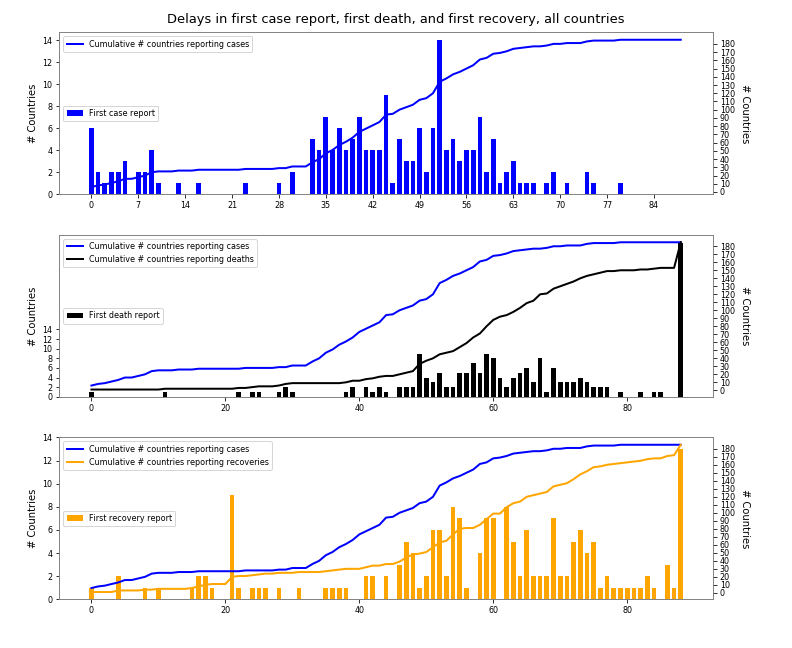
\includegraphics[width=\textwidth]{../tsam_Covid19_analysis/figures/tsam_Covid19_JHU_reportArrivals_AllCountries}
\end{minipage}%
\begin{minipage}{0.4\textwidth}
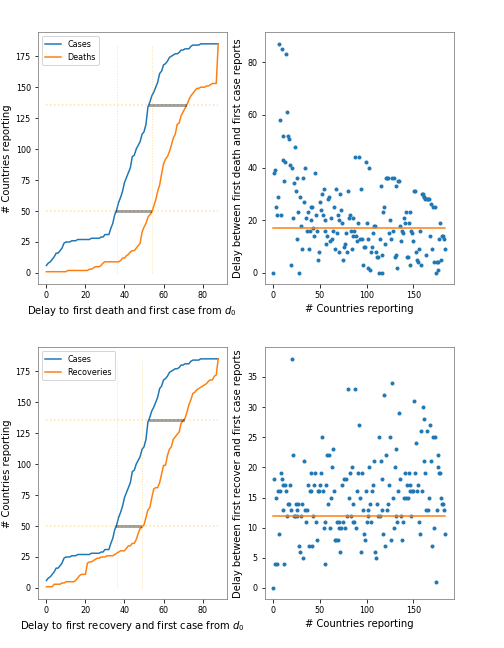
\includegraphics[width=\textwidth]
{../tsam_Covid19_analysis/figures/tsam_Covid19_JHU_delays_caseDeaths}
\end{minipage}%
\end{figure}
De esa forma también es posible medir el retraso entre reportes de casos y primera recuperación, que resulta ser de aproximadamente 12 días. 

\bigskip
La fatalidad en casos confirmados puede depender de una diversidad de factores como la calidad de los servicios de salud, y el acceso a dichos servicios, entre otros. 
Sin embargo, es posible observar algunas similitudes macroscópicas en el comportamiento de las defunciones por Covid-19 en lugares que podría pensarse que los fallecimientos presentarían comportamientos muy distintos , como China y Korea del Sur por un lado, o Italia, por otro. 
En Korea del Sur y China, el control es muy estricto y la cuantificación de casos ha sido masiva. 
En cambio en Italia, donde la estructura poblacional es distinta, ha habido más fallecimientos por Covid-19, y ha sido rebasado el sistema de salud al grado de tener que negar el uso de respiradores a la gente. 
Sin embargo, en los tres paises el cociente de fatalidad de casos (CFR por sus siglas en inglés) tiene muchas similitudes (\figref{fig:estimates}, panel izquierdo), que se pueden explotar para obtener las contribuciones relativas de los fallecimientos por Covid-19 (\figref{fig:reportArrivals}, panel derecho) por cada grupo de edad al total de muertes observadas, y usar esas estimaciones. 


%
\begin{figure}[h]
\caption{Estimaciones de fatalidad para México tomando en cuenta grupos de edad, con los datos de China, Korea del Sur, e Italia, calculado hasta el 11 de abril de 2020, y usando un factor de ajuste por subreporte igual a 1. }. \label{fig:estimates}
\begin{minipage}{0.6\textwidth}
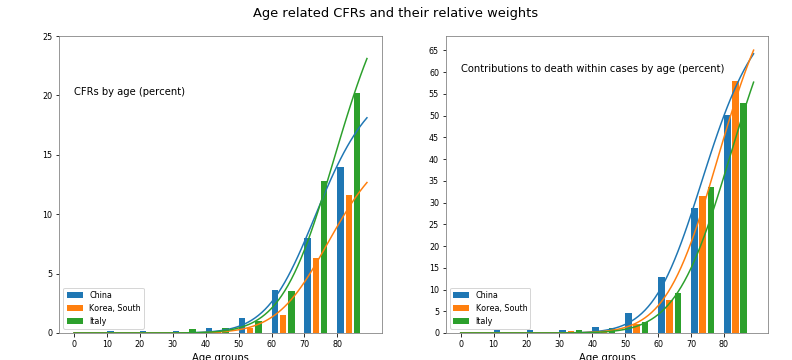
\includegraphics[width=\textwidth]{../tsam_Covid19_analysis/figures/tsam_Covid19_JHU_cfr+propDeathCases_ByAge_China+SKorea+Italy_OneFigure.png}
\end{minipage}%
\begin{minipage}{0.4\textwidth}
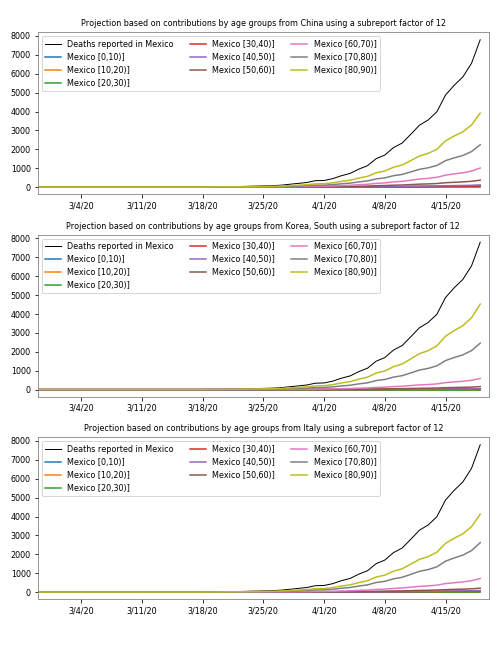
\includegraphics[width=\textwidth]
{../tsam_Covid19_analysis/figures/tsam_Covid19_JHU_cfr+propDeathCasesByAgeTS_EstimatesMexico_subReportFactor12.png}
\end{minipage}%
\end{figure}

Por su similitud, es posible usar los pesos relativos de las defunciones de los distintos grupos de edad y  hacer distintas predicciones para el caso de México (\figref{fig:estimates_sp}).


Las proyecciones obtenidas usando los datos de los distintos países son similares. Hay que tomar en cuenta que estos datos no han sido ajustados con respecto a subreporte. Por ejemplo, sin ajustar los datos por subreporte, la estimación del 11 de abril de 2020 es  de alrededor 150 muertes de adultos de más de 70 años en México. 
Usando un factor de ajuste por subreporte igual a 10, estaríamos estimando que el número de muertes por COVID-19 en México sería aproximadamente 1500. 


Es importante mencionar que estas estimaciones no toman en cuenta la estructura poblacional en México, o la de los países tomados para el análisis, pero esa información está implícita en los datos de dichos países. 





